\documentclass[10pt]{article}
\usepackage[utf8]{inputenc}
\usepackage[T1]{fontenc}
\usepackage{amsmath}
\usepackage{amsfonts}
\usepackage{amssymb}
\usepackage[version=4]{mhchem}
\usepackage{stmaryrd}
\usepackage{hyperref}
\hypersetup{colorlinks=true, linkcolor=blue, filecolor=magenta, urlcolor=cyan,}
\urlstyle{same}
\usepackage{graphicx}
\usepackage[export]{adjustbox}
\graphicspath{ {./images/} }

\title{The Effect of Visual Semantics and Aesthetics on User Experience }


\author{Ronak Prasad\\
Compiled January 15, 2023}
\date{}


\begin{document}
\maketitle


\begin{abstract}
Aesthetic principle not only concerns the perception of visual beauty, but most crucially, the cognitiveaffective responses derived from experiencing such stimuli. Despite this knowledge, user experience (UX) designers often prioritise beauty over intended end-user affect. This reversed order of prioritisation contradicts the sequential UX design process, leading to unexpected end-user perceptions and responses. The challenge in shaping UX before user interface (UI) design is that there first must be prior knowledge of aesthetic affect. A study with 1,782 worldwide participants was conducted evaluating affective user-responses to 43 atomic aesthetics using 153,252 data points and presented as affect ratings (ARs). Results demonstrated high affective resonance amongst aesthetics evaluated, suggesting aesthetic AR may be a viable method of improving the UX design process by influencing user perceptions, responses and actions at a non-conscious level. This is the first of a series of studies in the direction of Aesthetic Semantics $\odot 2023$ Optica Publishing Group
\href{http://dx.doi.org/10.1364/ao.XX.XXXXXX}{http://dx.doi.org/10.1364/ao.XX.XXXXXX}
\end{abstract}

\section{INTRODUCTION}
User experience (UX) designers tend to prioritise the creation of aesthetic appeal (visual beauty) [ 3 ] before the process of devising an intended end-user affect This can result in a disjoint between the expected end-user experience and actual end-user experience, leading to unanticipated user-responses. Aesthetic principle concerns much more than just the appeal of visual stimuli. Most crucially, it concerns the cognitive-affective responses derived from experiencing such sensory stimuli. The importance of affective experiences is why modern web design begins with UX strategy [5] , prior to user interface (UI) design. In its entirety, the UX "design" process relies on the aesthetic synergy of beauty and intended useraffect through the combination of initial UX research and associated UI design . The philosophy of aesthetics concerns how an observer perceives, interprets and responds to stimuli in relation to valence and other sensori-emotive values such as arousal. Ultimately, it is how an observer derives affective meaning (UX) from aesthetic stimuli (UI).

The difficulty for UX designers in shaping a desired user experience before constructing visual design, is that a designer must first understand what core perceptions already exist for potential aesthetics of choice.

\section{LITERATURE REVIEW}
Aesthetic semantics is an approach that aims to identify the core, most resonant affective interpretations of atomic-level visual aesthetics. In the space of the Web, these "atomic-level" aesthetics are the individual values within the properties of; colour, typeface and UI animation. Combined use of these atomic-level aesthetics is what forms the basis of UI objects such as animated UI buttons (i.e. a button can have a colour, text, and a hover animation). The atomic approach to aesthetic semantics is therefore crucial as a starting point, because it allows for evaluation of the most fundamental aspects of each property without compounded influence. This acts as one of the many control methods used in this research to help minimise the possibility of confounding variables. With this required atomic-level data, planned future research can accurately explore how atomic aesthetics may impact useraffect when they are grouped together to form UI elements, and then ultimately; full page templates.

Visual aesthetics form the building blocks of graphical user interface design. The three core aesthetic properties usually considered during the initial stage of UI design include; colour, typeface, and UI animation. It is the distinct values within these properties that are referred to as an "atomic" aesthetic i.e. an individual colour, specific font or single animation. The following sections discuss the aesthetic properties explored, why the atomic approach was taken and justifications behind the selection process.

To truly "design" an affective user experience, it is essential to understand exactly how UX and UI work together, how user perceptions are influenced by specific aesthetics of UI, and the necessary relationship between subjectivity and objectivity in HCI research. To properly investigate the challenges of affective UX design, it is also important to explore visual aesthetics from its most granular form (atoms) using the most justified models relative to this work. Through the atomic approach, mapping affective user-response to visual aesthetic becomes more feasibly achievable.

\section{A. Atomic Visual Web Semantics}
Normal and abnormal behaviors are defined using densitybased classification algorithms, such as local outlier factor and density-based spatial clustering of applications with noise, as previously described in (Hurst et al., 2020). The anomalous points are then validated by cross-checking with the corresponding data record (Hurst et al., 2020). After being labeled, a feature extraction process is conducted, which involves calculating the frequency, mean, mode, standard deviation, minimum, 5th percentile, 25th percentile, median, 75th percentile, 95 th percentile, maximum, and outlier score. The data is then consolidated and vectors are categorized as normal or anomalous. A supervised machine learning process is then used for anomaly detection. The dataset used in this research is unbalanced for classification, which is a common challenge in most real-world classification problems where the classes do not make up an equal portion of the dataset. Therefore, the research adhered to this data structure for the experiments instead of using techniques such as Synthetic Minority Over-sampling Technique (SMOTE) to balance the dataset prior to classification.
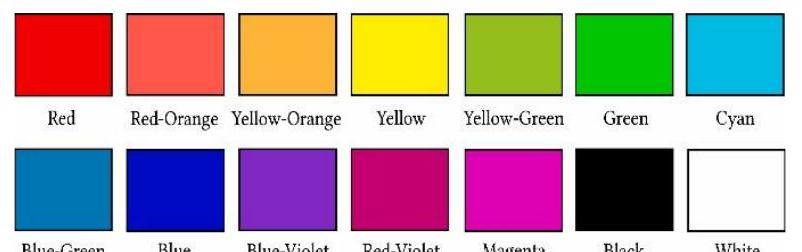
\includegraphics[max width=\textwidth, center]{2023_01_16_edd5388a973e00ef26e3g-2}

\begin{center}

\includegraphics[max width=\textwidth]{2023_01_16_edd5388a973e00ef26e3g-2(1)}
\end{center}

$\mathrm{Abc}$

$A b c$

$\frac{\mathrm{Abc}}{\text { Robbos Sab }}$

\begin{center}

\includegraphics[max width=\textwidth]{2023_01_16_edd5388a973e00ef26e3g-2(2)}
\end{center}

$\mathrm{Abc}$

Abc

Abc Abc

Aoc

Lato

Righteous

Patua One

Oleo Script

Courgette

\begin{center}

\includegraphics[max width=\textwidth]{2023_01_16_edd5388a973e00ef26e3g-2(3)}
\end{center}

$\mathrm{Abc}$

Abc

Abc

Yellowtail

Inconsolata

Source Code Pro Ubuntu Mono

\section{B. METHODOLOGY}
The algorithms chosen for the anomaly detection process include i) decision tree, ii) random decision forest and iii) Support Vector Machine (SVM). Decision trees are a wellknown classification tool for modeling and predicting decisions and their potential outcomes based on chance event outcomes. It works by using a binary splitting tech- nique, where feature dominance plays a crucial role inthe prediction outcome.Decision trees provide an effective benchmark experiment due to their popularity and efficiency.

\includegraphics[max width=\textwidth, center]{2023_01_16_edd5388a973e00ef26e3g-2(4)}

Random decision forests typically achieve a high predictive accuracy by generating bootstrapped trees. The final predicted

outcome is achieved by combining the results across all of the trees by using an average in regression/majority vote. The random forest approach offers an interesting comparison with the decision tree, as the decision tree makes its prediction from the entire dataset, whereas the random forest selects observations at random (and specific features) to build multiple C. Sample Table

Table 3 shows an example table.

Table 1. Colour Affect Rating (AR) Data Summary.

\begin{center}
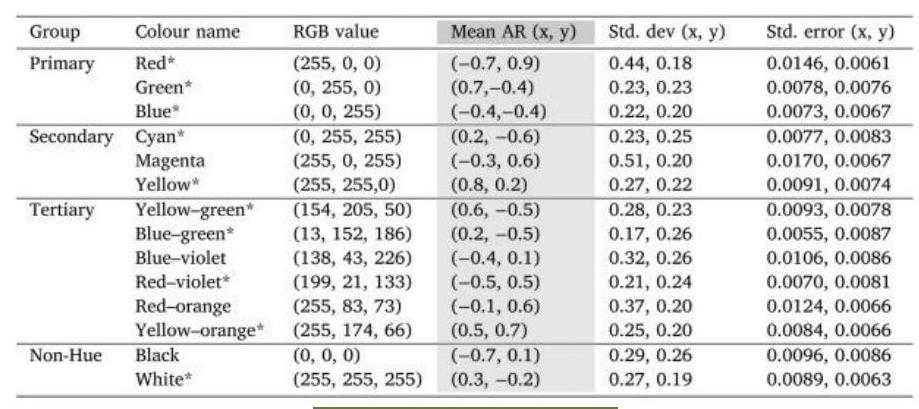
\includegraphics[max width=\textwidth]{2023_01_16_edd5388a973e00ef26e3g-2(5)}
\end{center}

Normal and Abnormal dataset distribution

\begin{center}
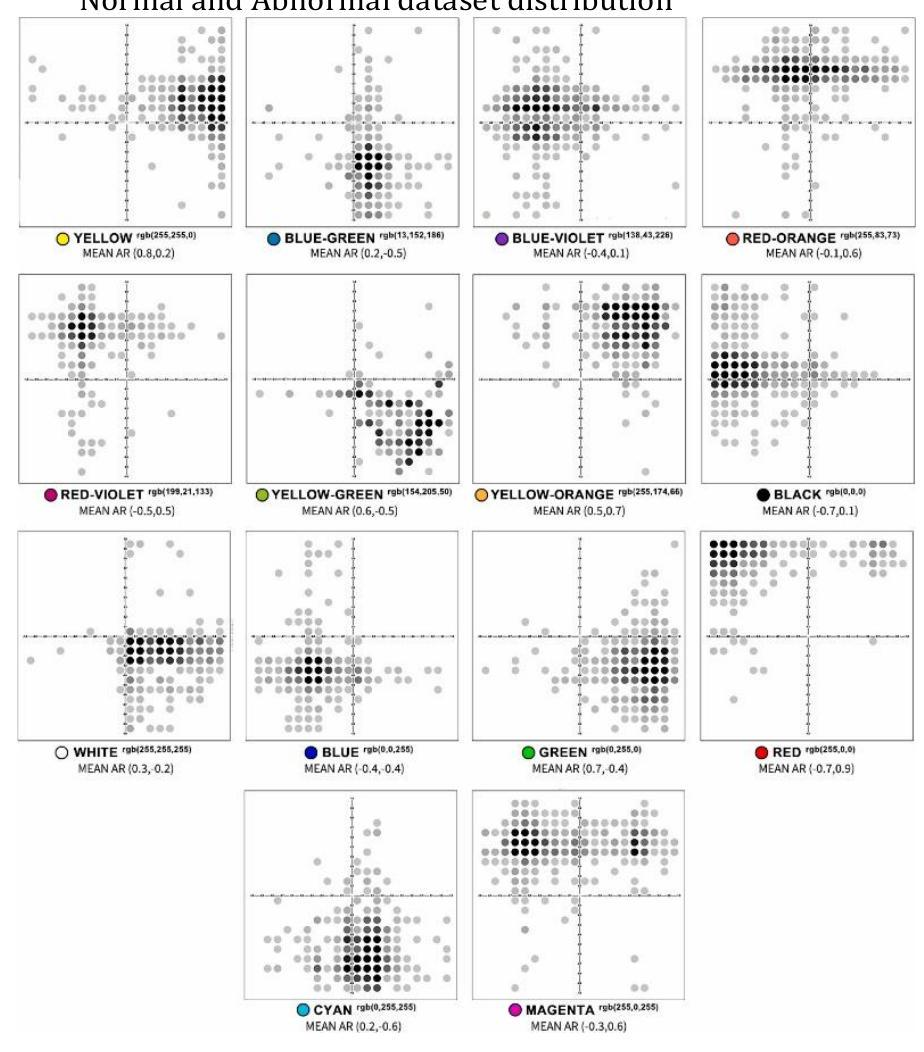
\includegraphics[max width=\textwidth]{2023_01_16_edd5388a973e00ef26e3g-2(6)}
\end{center}

Table 2. Decision tree confusion matrix

\begin{center}
\begin{tabular}{ccc}
\hline
Label & Predicted Anomaly & Predicted Normal \\
\hline
Anomaly(TrueAnomaly) & 38 & 1 \\
Normal(TrueNormal) & 69 & 5646 \\
\end{tabular}
\end{center}

decision trees. An SVM is primarily a discriminative classifier which is concerned with the optimal hyperplane calculation for categorizing data points. It is an ideal technique for highdimensional data and working with binary decisions. The experiments involve training the algorithms on all labels, converted to either normal or abnormal with outlier score

removed. The benefit of adopting this approach is that the challenge is a binary classification problem, i.e. normal compared with anomalous data.

\section{CONCLUSION}
The implementation of Electronic Health Records (EHR) has brought many benefits to the healthcare industry, such as increased efficiency, cost savings, and environmental benefits. However, these new systems also bring new risks. Advanced anomaly detection methods are crucial in maintaining the confidentiality, integrity, and availability of the data. In this paper, the authors proposed an anomaly detection method using three supervised learning classifiers to identify anomalous data access. The results showed that using a Support Vector Machine (SVM) was the most effective method. This study focuses on detecting internal threats based on abnormal behavior patterns when using EHRs. To the best of the authors' knowledge, this is the first time this methodology has been applied to this specific dataset with a focus on internal threat detection. In future research, the effectiveness of this approach in real-time situations will be evaluated, and deep learning methods will be used to improve the overall accuracy of anomaly detection predictions. The study will also use a larger dataset and improve the balance between anomalous and normal readings, and compare the results with this manuscript. Table 3. Random forest confusion matrix

\begin{center}
\begin{tabular}{ccc}
Label & Anomaly & Normal \\
\hline
Anomaly(TrueAnomaly) & 42 & 65 \\
Normal(TrueNormal) & 7 & 5640 \\
\hline
\end{tabular}
\end{center}

\section{REFERENCES}
\begin{enumerate}
  \item D. Chitimalla, K. Kondepu, L. Valcarenghi, M. Tornatore, and B. Mukher- jee, " $5 \mathrm{~g}$ fronthaul-latency and jitter studies of cpri over ethernet," J. Opt. Commun. Netw. 9, 172-182 (2017).

  \item Y.-H. Wen, J.-W. Ho, and K.-M. Feng, "Simultaneous all-optical trans- parent phase multiplexing/de-multiplexing based on fwm in a hnlf," in Optical Fiber Communication Conference, (Optica, 2022), p. W4D.1.

  \item Aesthetic semantics: Affect rating of atomic visual web aesthetics for use in affective user experience design \href{https://www.sciencedirect.com/science/article/abs/pii/S1071581922001392}{https://www.sciencedirect.com/science/article/abs/pii/S1071581922001392}

\end{enumerate}

\end{document}